\begin{enumerate}
\def\labelenumi{\arabic{enumi}.}
\item
  \protect\phantomsection\label{Phux1b0ux1a1ng_phuxe1p_thux1ef1c_hiux1ec7n}{}Các thành phần monitoring

  \begin{enumerate}
  \def\labelenumii{\arabic{enumii}.}
  \item
    JSON file
  \item
    Prometheus
  \item
    Grafana
  \end{enumerate}
\end{enumerate}

\begin{enumerate}
\def\labelenumi{\arabic{enumi}.}
\item
  PHƯƠNG PHÁP THỰC HIỆN

  \begin{enumerate}
  \def\labelenumii{\arabic{enumii}.}
  \item
    \protect\phantomsection\label{Cuxf4ng_cux1ee5_sux1eed_dux1ee5ng}{}Công cụ sử dụng

    \begin{enumerate}
    \def\labelenumiii{\arabic{enumiii}.}
    \item
      \protect\phantomsection\label{Linux_}{}Proxmox
    \item
      \protect\phantomsection\label{Docker_Bench_Security}{}Docker Bench Security
    \end{enumerate}
  \end{enumerate}
\end{enumerate}

\begin{quote}
Docker Bench Security là một script mã nguồn mở do Docker Inc. phát triển. Công cụ này tự động kiểm tra các Benchmark theo chuẩn CIS Docker Benchmark trên môi trường Docker đang chạy, cho phép quản trị viên nhanh chóng đánh giá mức độ tuân thủ bảo mật của hệ thống.

Docker Bench Security hoạt động bằng cách mount các thư mục hệ thống của host vào container kiểm tra, sau đó thực thi các bài kiểm tra tương ứng với từng Section trong CIS Docker Benchmark. Với mỗi mục kiểm tra, công cụ trả về một trong ba kết quả:
\end{quote}

\begin{itemize}
\item
  PASS: Cấu hình hiện tại đáp ứng đúng khuyến nghị.
\item
  WARN: Cấu hình không đáp ứng khuyến nghị, cần khắc phục.
\item
  INFO: Thông tin bổ sung, cần xem xét thủ công.
\end{itemize}

\begin{quote}
Kết quả được xuất ra terminal và lưu đồng thời vào hai file log: docker-bench- security.log (dạng văn bản) và docker-bench-security.log.json (dạng JSON) để phục vụ phân tích hoặc tích hợp vào pipeline CI/CD.

Tool này sẽ được sử dụng để đối chứng kết quả với audition tự làm và cho việc remediation.
\end{quote}

Docker Bench Security https://github.com/docker/docker-bench-security\protect\phantomsection\label{_bookmark25}{}

\begin{enumerate}
\def\labelenumi{\arabic{enumi}.}
\item
\item
  \begin{enumerate}
  \def\labelenumii{\arabic{enumii}.}
  \item
    \begin{enumerate}
    \def\labelenumiii{\arabic{enumiii}.}
    \item
    \item
    \item
      \textbf{Ansible}
    \end{enumerate}
  \end{enumerate}
\end{enumerate}

\begin{quote}
Sử dụng Ansible để tự động hóa và cải thiện Docker phù hợp với Benchmark sau khi thực hiện manual:
\end{quote}

\begin{itemize}
\item
  Host: Đích đến sẽ là Docker
\item
  Các file yaml/yml sẽ là các mục từ 1 đến 6.
\end{itemize}

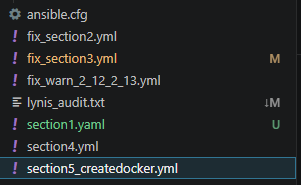
\includegraphics[width=3.13585in,height=1.92735in]{images/media/image3.png}

Sẽ có 2 loại task: automatic và manual:

\begin{itemize}
\item
  Với các task có thể automatic được, khi chạy lệnh ansible-playbook thì sẽ chạy các ask cần thiết, điều chỉnh file, chạy container tự động.
\item
  Với các task manual, thường sẽ phải kiểm tra hoặc thực hiện bằng tay.

  \begin{enumerate}
  \def\labelenumi{\arabic{enumi}.}
  \item
    \textbf{Prometheus}
  \item
    \textbf{Grafana}
  \end{enumerate}

  \begin{enumerate}
  \def\labelenumi{\arabic{enumi}.}
  \item
    \textbf{Bảng các hoạt động cần thực hiện}
  \end{enumerate}
\end{itemize}

{\def\LTcaptype{none} % do not increment counter
\begin{longtable}[]{@{}|
  >{\raggedright\arraybackslash}p{(\linewidth - 8\tabcolsep - 5\arrayrulewidth) * \real{0.0772}}|
  >{\raggedright\arraybackslash}p{(\linewidth - 8\tabcolsep - 5\arrayrulewidth) * \real{0.2973}}|
  >{\raggedright\arraybackslash}p{(\linewidth - 8\tabcolsep - 5\arrayrulewidth) * \real{0.2208}}|
  >{\raggedright\arraybackslash}p{(\linewidth - 8\tabcolsep - 5\arrayrulewidth) * \real{0.4047}}|@{}}
\hline
\begin{minipage}[b]{\linewidth}\raggedright
\textbf{Phần}
\end{minipage} & \begin{minipage}[b]{\linewidth}\raggedright
\textbf{Benchmark}
\end{minipage} & \begin{minipage}[b]{\linewidth}\raggedright
\textbf{Loại(Auto/Manual)}
\end{minipage} & \begin{minipage}[b]{\linewidth}\raggedright
\textbf{\textbf{Nội dung}}
\end{minipage} \\
\hline
\endhead
\endlastfoot
\multirow{19}{=}{\textbf{1}} & \textbf{Phân vùng riêng cho các container} & \textbf{Manual} & \textbf{Đảm bảo tạo phân vùng riêng biệt cho các container. Toàn bộ dữ liệu Docker được lưu tại /var/lib/docker; cần mount điểm này vào một phân vùng riêng để tránh ảnh hưởng đến hệ thống khi đĩa đầy.} \\
\hline
& \textbf{Chỉ cho trusted user kiểm soát Docker Daemon} & \textbf{Manual} & \textbf{Chỉ những người dùng đáng tin cậy mới được phép kiểm soát Docker daemon. Docker daemon socket mặc định thuộc sở hữu của root và nhóm docker; quyền truy cập không kiểm soát có thể dẫn đến leo thang đặc quyền.} \\
\hline
& \textbf{Cấu hình kiểm tra nhật ký cho Docker Daemon} & \textbf{Automated} & \textbf{Cấu hình audit cho Docker daemon. Kiểm tra log hoạt động của Docker daemon giúp phát hiện hành vi bất thường và đảm bảo tuân thủ chính sách bảo mật.} \\
\hline
& \textbf{Audit folder /run/containerd} & \textbf{Manual} & \textbf{Cấu hình audit cho thư mục /run/containerd. Việc giám sát thư mục này đảm bảo theo dõi được các hoạt động liên quan đến containerd runtime.} \\
\hline
& \textbf{Audit folder /var/lib/docker} & \textbf{Manual} & \textbf{Cấu hình audit cho thư mục /var/lib/docker. Thư mục này lưu trữ toàn bộ dữ liệu Docker bao gồm image và container; cần được giám sát chặt chẽ.} \\
\hline
& \textbf{Audit folder /etc/Docker} & \textbf{Automated} & \textbf{Cấu hình audit cho thư mục /etc/docker. Đây là nơi lưu các tệp cấu hình TLS và chứng chỉ của Docker; cần kiểm soát mọi thay đổi.} \\
\hline
& \textbf{Audit docker.service} & \textbf{Automated} & \textbf{Cấu hình audit cho tệp docker.service (nếu có). Giám sát tệp service giúp phát hiện thay đổi trái phép đối với cấu hình khởi động Docker daemon.} \\
\hline
& \textbf{Audt containerd.sock} & \textbf{Automated} & \textbf{Cấu hình audit cho socket containerd.sock (nếu có). Socket này là điểm giao tiếp với containerd; mọi truy cập cần được ghi nhận.} \\
\hline
& \textbf{Audit docker.sock} & \textbf{Automated} & \textbf{Cấu hình audit cho socket docker.sock (nếu có). Docker socket là giao diện chính để tương tác với Docker daemon; cần theo dõi toàn bộ hoạt động.} \\
\hline
& \textbf{Audt /etc/default/docker} & \textbf{Automated} & \textbf{Cấu hình audit cho tệp /etc/default/docker (nếu có). Tệp này chứa các biến môi trường và tùy chọn khởi động cho Docker daemon.} \\
\hline
& \textbf{Audit /etc/docker/daemon.json} & \textbf{Automated} & \textbf{Cấu hình audit cho tệp /etc/docker/daemon.json (nếu có). Đây là tệp cấu hình chính của Docker daemon; mọi thay đổi cần được theo dõi.} \\
\hline
& \textbf{Audit /etc/containerd/config.toml} & \textbf{Automated} & \textbf{Cấu hình audit cho tệp /etc/containerd/config.toml (nếu có). Tệp cấu hình của containerd cần được giám sát để phát hiện thay đổi trái phép.} \\
\hline
& \textbf{Aduti /etc/sysconfig/docker} & \textbf{Automated} & \textbf{Cấu hình audit cho tệp /etc/sysconfig/docker (nếu có). Tệp cấu hình hệ thống cho Docker trên các distro dùng sysconfig (như RHEL/CentOS).} \\
\hline
& \textbf{Audit /usr/bin/containerd-shim} & \textbf{Automated} & \textbf{Cấu hình audit cho tệp /usr/bin/containerd-shim (nếu có). Binary này là thành phần trung gian giữa containerd và container runtime; cần kiểm tra tính toàn vẹn.} \\
\hline
& \textbf{Audit /usr/bin/containerd-shim-runc-v1} & \textbf{Automated} & \textbf{Cấu hình audit cho tệp /usr/bin/containerd-shim-runc-v1 (nếu có). Đây là binary shim cho runc v1; cần đảm bảo mọi truy cập được ghi nhận.} \\
\hline
& \textbf{Audit /usr/bin/containerd-shim-runc-v2} & \textbf{Manual} & \textbf{Cấu hình audit cho tệp /usr/bin/containerd-shim-runc-v2 (nếu có). Binary shim cho runc v2; cần kiểm soát và ghi lại mọi thay đổi.} \\
\hline
& \textbf{Audit /usr/bin/runc} & \textbf{Automated} & \textbf{Cấu hình audit cho tệp /usr/bin/runc (nếu có). runc là container runtime cấp thấp; bất kỳ thay đổi nào đối với binary này đều có thể ảnh hưởng nghiêm trọng đến bảo mật.} \\
\hline
& \textbf{Đảm báo bảo mật cho container} & \textbf{Manual} & \textbf{Đảm bảo máy chủ container đã được hardening đúng cách. Máy chủ Docker cần được cấu hình bảo mật chặt chẽ bao gồm vá lỗi, tắt dịch vụ không cần thiết và tuân theo các tiêu chuẩn bảo mật hệ thống.} \\
\hline
& \textbf{Đảm bảo phiên bản mới cho Docker} & \textbf{Manual} & \textbf{Đảm bảo Docker đang sử dụng phiên bản mới nhất. Các phiên bản mới thường khắc phục lỗ hổng bảo mật; cần theo dõi và nâng cấp định kỳ.} \\
\hline
\multirow{19}{=}{\textbf{2}} & \textbf{Chạy docker daemon tránh quyền root} & \textbf{Manual} & \textbf{Chạy Docker daemon với chế độ rootless nếu có thể. Rootless mode thực thi Docker daemon và container trong user namespace, không yêu cầu quyền root, giảm thiểu rủi ro leo thang đặc quyền.} \\
\hline
& \textbf{Network trafic được đặt hạn chế giữa các container ở default bridge} & \textbf{Manual} & \textbf{Hạn chế lưu lượng mạng giữa các container trên default bridge network. Mặc định tất cả container trên cùng host có thể giao tiếp; cần giới hạn bằng cách sử dụng tùy chọn -\/-icc=false.} \\
\hline
& \textbf{Logging level set ở ``info''} & \textbf{Manual} & \textbf{Đặt mức độ log của Docker daemon ở mức \textquotesingle info\textquotesingle. Mức log \textquotesingle info\textquotesingle{} cung cấp đủ thông tin để giám sát mà không gây quá tải; tránh dùng \textquotesingle debug\textquotesingle{} trong môi trường production.} \\
\hline
& \textbf{Docker được quyền thay đổi iptables} & \textbf{Manual} & \textbf{Cho phép Docker daemon thay đổi rules iptables. Docker cần được quyền quản lý iptables để thiết lập kết nối mạng cho container; không nên vô hiệu hóa tính năng này.} \\
\hline
& \textbf{Đảm bảo không sử dụng registry không an toàn} & \textbf{Manual} & \textbf{Không sử dụng insecure registry. Docker mặc định coi registry là an toàn; việc cấu hình insecure-registries có thể dẫn đến tải image từ nguồn không tin cậy qua kết nối không mã hóa.} \\
\hline
& \textbf{Đảm bảo không sử dụng trình điều khiển aufs} & \textbf{Manual} & \textbf{Không sử dụng storage driver aufs. aufs là driver lỗi thời, không được hỗ trợ trên nhiều kernel hiện đại và có thể gây ra các vấn đề bảo mật; nên dùng overlay2.} \\
\hline
& \textbf{Đảm bảo không dùng devicemapper} & \textbf{Manual} & \textbf{Không sử dụng storage driver devicemapper. devicemapper ở chế độ loop-lvm không phù hợp cho production do hiệu suất kém và các rủi ro bảo mật tiềm ẩn.} \\
\hline
& \textbf{Đảm bảo xác thực TLS cho Docker Daemon} & \textbf{Manual} & \textbf{Cấu hình xác thực TLS cho Docker daemon khi mở qua TCP. Kết nối TCP tới Docker daemon cần được bảo mật bằng TLS mutual authentication để ngăn chặn truy cập trái phép.} \\
\hline
& \textbf{Đảm bảo giới hạn ulimit mặc định} & \textbf{Manual} & \textbf{Cấu hình giới hạn ulimit mặc định phù hợp. Giới hạn ulimit kiểm soát tài nguyên hệ thống mà container có thể sử dụng; cần đặt giá trị hợp lý để tránh lạm dụng tài nguyên.} \\
\hline
& \textbf{Hỗ trợ user namespace} & \textbf{Manual} & \textbf{Bật hỗ trợ user namespace trong Docker daemon. User namespace cho phép ánh xạ user trong container sang user không có quyền trên host, giảm thiểu rủi ro nếu container bị xâm phạm.} \\
\hline
& \textbf{Cgroup sử dụng được xác nhận} & \textbf{Manual} & \textbf{Xác nhận cgroup đang sử dụng là phù hợp. Tùy chọn -\/-cgroup-parent cho phép đặt cgroup cha mặc định; nếu không có yêu cầu đặc biệt nên để mặc định.} \\
\hline
& \textbf{Đảm bảo device size không thay đổi trừ khi cần thiết} & \textbf{Manual} & \textbf{Không thay đổi base device size nếu không cần thiết. Thay đổi kích thước thiết bị cơ sở có thể ảnh hưởng đến bảo mật và hiệu suất; chỉ thực hiện khi thực sự cần.} \\
\hline
& \textbf{Đảm bảo authorization cho Docker client} & \textbf{Manual} & \textbf{Bật authorization plugin cho các lệnh Docker client. Sử dụng plugin phân quyền gốc của Docker hoặc cơ chế bên thứ ba để kiểm soát quyền truy cập vào Docker daemon.} \\
\hline
& \textbf{Đảm bảo container bj hạn chế không cho quyền mới} & \textbf{Manual} & \textbf{Hạn chế container không được phép nhận thêm quyền mới. Cấu hình -\/-no-new-privileges ngăn container leo thang đặc quyền thông qua suid hoặc sgid.} \\
\hline
& \textbf{Đảm bảo container có live restore} & \textbf{Manual} & \textbf{Bật tính năng live restore cho Docker daemon. -\/-live-restore đảm bảo container tiếp tục chạy khi Docker daemon khởi động lại, tăng tính sẵn sàng của dịch vụ.} \\
\hline
& \textbf{Đảm bảo có log cho đăng nhập gần và từ xa} & \textbf{Manual} & \textbf{Cấu hình centralized và remote logging. Logging tập trung giúp quản lý, phân tích log từ nhiều container và phát hiện sự cố bảo mật kịp thời.} \\
\hline
& \textbf{Đảm bảo Userland Proxy đã tắt} & \textbf{Manual} & \textbf{Tắt Userland Proxy nếu không cần thiết. Docker userland proxy xử lý chuyển tiếp cổng; khi hairpin NAT khả dụng, proxy này là dư thừa và có thể bị tắt để giảm bề mặt tấn công.} \\
\hline
& \textbf{Đảm bảo daemon-wide custom seccomp profile được thiết đặt} & \textbf{Manual} & \textbf{Áp dụng custom seccomp profile ở cấp daemon nếu phù hợp. Seccomp profile tùy chỉnh giúp hạn chế các system call mà container có thể thực hiện, tăng cường bảo mật.} \\
\hline
& \textbf{Đảm bảo các tính năng thử nghiệm không được triển khai trong môi trường sản xuất} & \textbf{Manual} & \textbf{Không bật experimental features trong môi trường production. Các tính năng thử nghiệm chưa được kiểm tra đầy đủ và có thể chứa lỗ hổng bảo mật chưa được vá.} \\
\hline
\multirow{14}{=}{\textbf{3}} & \textbf{Đảm bảo quyền root:root cho docker.service} & \textbf{Automated} & \textbf{Đảm bảo file docker.service thuộc sở hữu của root:root. Quyền sở hữu không đúng có thể cho phép người dùng không có quyền sửa đổi cấu hình service Docker.} \\
\hline
& \textbf{Đảm bảo docker.service cho quyền hợp lý} & \textbf{Automated} & \textbf{Đảm bảo file docker.service có file permissions được đặt thành 644 hoặc hạn chế hơn. Quyền truy cập quá rộng có thể bị lợi dụng để sửa đổi cấu hình Docker daemon.} \\
\hline
& \textbf{Đảm bảo quyền sở hữu của docker.socket được đặt thành root:root} & \textbf{Automated} & \textbf{Đảm bảo file docker.socket thuộc sở hữu root:root. Docker socket là điểm truy cập chính tới daemon; quyền sở hữu không đúng có thể dẫn đến truy cập trái phép.} \\
\hline
& \textbf{Đảm bảo quyền truy cập tệp docker.socket được đặt thành 644 hoặc hạn chế} & \textbf{Automated} & \textbf{Đảm bảo file docker.socket có permissions 644 hoặc hạn chế hơn. Giới hạn quyền truy cập vào socket file ngăn chặn người dùng không được phép tương tác với Docker daemon.} \\
\hline
& \textbf{Đảm bảo quyền sỡ hữu thư mục /etc/docker được đặt thành root:root} & \textbf{Automated} & \textbf{Đảm bảo thư mục /etc/docker thuộc sở hữu root:root. Thư mục này chứa chứng chỉ TLS và cấu hình nhạy cảm; cần được bảo vệ chặt chẽ.} \\
\hline
& \textbf{Đảm bảo quyền truy cập thư mục /etc/docker được đặt thành 755 hoặc hạn chế} & \textbf{Automated} & \textbf{Đảm bảo thư mục /etc/docker có permissions 755 hoặc hạn chế hơn. Quyền truy cập thư mục cấu hình cần được kiểm soát để tránh truy cập trái phép.} \\
\hline
& \textbf{Đảm bảo quyền truy cập tệ docker.socker được đặt thành 644 hoặc hạn chế} & \textbf{Automated} & \textbf{Kiểm tra lại permissions của docker.socket file là 644 hoặc hạn chế hơn để đảm bảo không có quyền ghi thừa.} \\
\hline
& \textbf{Đảm bảo quyền root:root cho sỡ hữu tệp chứng chỉ} & \textbf{Manual} & \textbf{Đảm bảo các file chứng chỉ registry (thường trong /etc/docker/certs.d/) thuộc sở hữu root:root. Chứng chỉ không được bảo vệ có thể bị giả mạo hoặc đánh cắp.} \\
\hline
& \textbf{Đảm bảo quyền truy cập chứng trí registry được đặt thành 444 hoặc hạn chế hơn} & \textbf{Manual} & \textbf{Đảm bảo các file chứng chỉ registry có permissions 444 hoặc hạn chế hơn. Chứng chỉ chỉ nên được đọc, không được phép ghi hay thực thi bởi bất kỳ ai.} \\
\hline
& \textbf{Đảm bảo quyền sỡ hữu Docker server là root:root và file permission 4444} & \textbf{Manual} & \textbf{Đảm bảo file Docker server certificate (-\/-tlscert) thuộc sở hữu root:root với permissions 444. Certificate server cần được bảo vệ để đảm bảo tính xác thực của daemon.} \\
\hline
& \textbf{Đảm bảo quyền Docker socker file ownership là root:docker và để file permission 660} & \textbf{Automated} & \textbf{Đảm bảo Docker socket file thuộc sở hữu root:docker với permissions 660. Cấu hình này cho phép nhóm docker truy cập socket trong khi ngăn chặn người dùng không có quyền.} \\
\hline
& \textbf{Đảm bảo quyền daemon.json là root:root và file permssion 644} & \textbf{Manual} & \textbf{Đảm bảo file daemon.json (nếu có) thuộc sở hữu root:root với permissions 644. File cấu hình daemon chứa các thiết lập nhạy cảm cần được bảo vệ.} \\
\hline
& \textbf{Đảm bảo quyền /etc/sysconfig/docker là root:root và file permission 644} & \textbf{Manual} & \textbf{Đảm bảo file /etc/sysconfig/docker thuộc sở hữu root:root với permissions 644. File cấu hình hệ thống này chứa các tùy chọn môi trường cho Docker daemon.} \\
\hline
& \textbf{Đảm bảo Containered socket có quyền là root:root và file permission 660} & \textbf{Automated} & \textbf{Đảm bảo Containerd socket file thuộc sở hữu root:root với permissions 660 hoặc hạn chế hơn. Kiểm soát quyền truy cập socket containerd ngăn chặn tương tác trái phép với runtime.} \\
\hline
\multirow{9}{=}{\textbf{4}} & \textbf{Phải có container tạo, chạy trong trusted base images và không có package dư thừa không cần thiết được tải về.} & \textbf{Manual} & \textbf{Container phải được tạo từ trusted base images và không chứa package không cần thiết. Sử dụng image tin cậy từ nguồn chính thống, giảm thiểu attack surface bằng cách loại bỏ các gói thừa.} \\
\hline
& \textbf{Đảm bảo image được scan và phải có security patches} & \textbf{Manual} & \textbf{Quét image thường xuyên và rebuild để bao gồm các bản vá bảo mật. Image cần được scan định kỳ để phát hiện CVE và rebuild với patches mới nhất.} \\
\hline
& \textbf{Phải có HEALTHCHECK instruction} & \textbf{Manual} & \textbf{Thêm HEALTHCHECK instruction vào Dockerfile. HEALTHCHECK giúp Docker tự động kiểm tra tình trạng container đang chạy, phát hiện sự cố kịp thời.} \\
\hline
& \textbf{Phải có update instruction và không sử dụng một mình trong Dockerfiles} & \textbf{Manual} & \textbf{Không sử dụng lệnh update (như apt-get update) một mình trong Dockerfile. Lệnh update độc lập có thể cache lại và không đảm bảo cài đặt phiên bản mới nhất khi build.} \\
\hline
& \textbf{Không cung cấp quyền Setuid và Getuid} & \textbf{Manual} & \textbf{Loại bỏ các quyền setuid và setgid khỏi image. Bit setuid/setgid có thể bị khai thác để leo thang đặc quyền trong container; cần loại bỏ khi không cần thiết.} \\
\hline
& \textbf{Dùng COPY thay vì ADD} & \textbf{Manual} & \textbf{Sử dụng instruction COPY thay vì ADD trong Dockerfile. COPY chỉ sao chép file cục bộ, trong khi ADD có thêm tính năng ngầm (giải nén, tải URL) có thể gây ra rủi ro bảo mật.} \\
\hline
& \textbf{Secrets không được bỏ vào Dockerfiles} & \textbf{Manual} & \textbf{Không lưu trữ secrets (password, key, token) trong Dockerfile. Secrets trong Dockerfile sẽ bị lộ trong image layers và có thể bị trích xuất bởi bất kỳ ai có quyền truy cập image.} \\
\hline
& \textbf{Các package phải chính thống khi tải về} & \textbf{Manual} & \textbf{Chỉ cài đặt các package đã được xác minh tính xác thực. Kiểm tra chữ ký và tính toàn vẹn của package trước khi cài đặt để tránh cài phần mềm độc hại.} \\
\hline
& \textbf{Các signed artifacts phải được kiểm chứng} & \textbf{Manual} & \textbf{Xác thực chữ ký của tất cả artifacts trước khi upload lên package registry. Đảm bảo tính toàn vẹn và nguồn gốc của artifacts trong chuỗi cung ứng phần mềm.} \\
\hline
\multirow{28}{=}{\textbf{5}} & \textbf{Không bật swarm mode nếu không cần thiết} & \textbf{Manual} & \textbf{Không bật Docker Swarm mode trừ khi cần thiết. Swarm mode mở thêm các cổng mạng và dịch vụ; nếu không sử dụng clustering nên tắt để giảm bề mặt tấn công.} \\
\hline
& \textbf{Bật AppArmor Profile} & \textbf{Manual} & \textbf{Bật AppArmor profile cho container (nếu hệ thống hỗ trợ). AppArmor là hệ thống bảo mật Linux giúp giới hạn khả năng của tiến trình trong container, ngăn chặn hành vi độc hại.} \\
\hline
& \textbf{Phải có SELinux} & \textbf{Manual} & \textbf{Cấu hình SELinux security options cho container (nếu hệ thống hỗ trợ). SELinux cung cấp mandatory access control, hạn chế quyền truy cập của container vào tài nguyên hệ thống.} \\
\hline
& \textbf{Linux Kernel phải để chế độ hạn chế trong containers} & \textbf{Manual} & \textbf{Hạn chế Linux kernel capabilities trong container. Docker mặc định chạy với tập capabilities giới hạn; chỉ thêm capabilities thực sự cần thiết và loại bỏ những capabilities không dùng.} \\
\hline
& \textbf{Không sử dụng privileged container} & \textbf{Manual} & \textbf{Không sử dụng -\/-privileged flag cho container. Container privileged có toàn bộ kernel capabilities của host và có thể thoát khỏi container; chỉ dùng khi thực sự bắt buộc.} \\
\hline
& \textbf{Không mount các host system cần bảo vệ chặt trong container} & \textbf{Manual} & \textbf{Không mount các thư mục nhạy cảm của host (/, /boot, /dev, /etc, /lib, /proc, /sys, /usr) vào container. Mount các thư mục này có thể cho phép container truy cập và sửa đổi hệ thống host.} \\
\hline
& \textbf{SSHD không chạy trong containers} & \textbf{Manual} & \textbf{Không chạy SSH daemon bên trong container. Thay vào đó, sử dụng docker exec để vào container. Chạy SSHD trong container làm phức tạp quản lý key và tăng attack surface.} \\
\hline
& \textbf{Không chạy port đặc quyền trong container} & \textbf{Manual} & \textbf{Không map các privileged ports (\textless{} 1024) vào container. Các port đặc quyền yêu cầu quyền root; việc map chúng vào container có thể tạo ra rủi ro bảo mật.} \\
\hline
& \textbf{Chỉ chạy port cần thiết cho container} & \textbf{Manual} & \textbf{Chỉ mở những port thực sự cần thiết cho container. Mỗi port mở thêm là một điểm tấn công tiềm ẩn; cần review và đóng những port không sử dụng.} \\
\hline
& \textbf{Bảo mật network namespace} & \textbf{Manual} & \textbf{Không chia sẻ host network namespace với container (-\/-net=host). Chế độ host networking loại bỏ cô lập mạng, cho phép container truy cập trực tiếp vào network stack của host.} \\
\hline
& \textbf{Sử dụng tài nguyên hợp lý: Memory usage và CPU priority(5.11, 5.12)} & \textbf{Manual} & \textbf{Giới hạn memory usage và CPU priority cho container. Không giới hạn tài nguyên có thể dẫn đến một container tiêu thụ hết tài nguyên host (DoS); cần đặt -\/-memory và -\/-cpu-shares phù hợp.} \\
\hline
& \textbf{Để filesystem của container's ở quyền ``read only''} & \textbf{Manual} & \textbf{Mount root filesystem của container ở chế độ read-only (-\/-read-only). Ngăn chặn ghi vào filesystem container giúp bảo vệ tính toàn vẹn của image và hạn chế tấn công persistence.} \\
\hline
& \textbf{Mạng lưu thông phải đến một interface được đặt} & \textbf{Manual} & \textbf{Bind incoming container traffic vào một host interface cụ thể. Thay vì bind 0.0.0.0, chỉ định interface cụ thể để kiểm soát traffic vào container và giảm exposure.} \\
\hline
& \textbf{Có chính sách ``on-failure'' thì khởi động lại với giá trị 5} & \textbf{Manual} & \textbf{Đặt restart policy \textquotesingle on-failure\textquotesingle{} với giá trị tối đa 5 lần. Chính sách này đảm bảo container tự khởi động lại khi gặp lỗi nhưng không chạy vô hạn khi có vấn đề nghiêm trọng.} \\
\hline
& \textbf{Bảo mật Host's process namespace và IPC namespace(5.16, 5.17)} & \textbf{Manual} & \textbf{Không chia sẻ PID namespace và IPC namespace của host với container. Chia sẻ các namespace này cho phép container nhìn thấy và tương tác với tiến trình/IPC của host, phá vỡ cô lập.} \\
\hline
& \textbf{Host Devices không nên tương tác chung với containers} & \textbf{Manual} & \textbf{Không expose host devices trực tiếp vào container trừ khi thực sự cần. Truy cập trực tiếp vào hardware của host có thể bị lợi dụng để thực hiện các cuộc tấn công đặc quyền.} \\
\hline
& \textbf{Phải có default limit overwritten trong lúc chạy nếu cần thiết} & \textbf{Manual} & \textbf{Ghi đè default ulimit khi chạy container nếu cần thiết. Các giới hạn tài nguyên cần được điều chỉnh phù hợp với yêu cầu của từng container để cân bằng bảo mật và hiệu năng.} \\
\hline
& \textbf{Để mount propagation và host's UTS namespace bí mật(5.20,5.21)} & \textbf{Manual} & \textbf{Không đặt mount propagation ở chế độ shared và không chia sẻ UTS namespace của host. Shared mount propagation có thể cho phép container ảnh hưởng đến mount point của host; UTS namespace lộ hostname của host.} \\
\hline
& \textbf{Chế độ của default seccomp profile không tắt} & \textbf{Manual} & \textbf{Không vô hiệu hóa default seccomp profile. Seccomp lọc system calls của container; tắt seccomp để lộ toàn bộ kernel syscall interface và tăng rủi ro kernel exploit.} \\
\hline
& \textbf{Khi sử dụng docker exec commands, không sử dụng quyền priviledged option hoặc user=root(5.23,5.24)} & \textbf{Manual} & \textbf{Không dùng -\/-privileged hoặc -\/-user=root với lệnh docker exec. Các tùy chọn này cấp quyền cao nhất khi vào container đang chạy và có thể bị lạm dụng để thoát khỏi sandbox.} \\
\hline
& \textbf{Phải có cgroup usage} & \textbf{Manual} & \textbf{Xác nhận cgroup usage khi chạy container. Đảm bảo container chạy trong cgroup đã được xác định để kiểm soát và giám sát tài nguyên đúng cách.} \\
\hline
& \textbf{Container chỉ cho quyền cần thiết và không thêm quyền không cần thiết} & \textbf{Manual} & \textbf{Hạn chế container không được nhận thêm đặc quyền (-\/-security-opt=no-new-privileges). Ngăn chặn leo thang đặc quyền thông qua suid/sgid bits trong runtime.} \\
\hline
& \textbf{Container health luôn chạy} & \textbf{Manual} & \textbf{Kiểm tra container health khi chạy bằng -\/-health-cmd nếu image không có HEALTHCHECK. Giám sát tình trạng container runtime giúp phát hiện và xử lý sự cố kịp thời.} \\
\hline
& \textbf{Docker command phải sử dụng lệnh mới nhất của image} & \textbf{Manual} & \textbf{Luôn sử dụng image version mới nhất từ repository. Sử dụng image cũ đã cache có thể bỏ qua các bản vá bảo mật quan trọng đã được cập nhật trong image mới.} \\
\hline
& \textbf{PIDs cgroup limit phải được sử dụng} & \textbf{Manual} & \textbf{Sử dụng -\/-pids-limit flag khi chạy container. Giới hạn số lượng process trong container ngăn chặn tấn công fork bomb và bảo vệ host khỏi cạn kiệt tài nguyên PID.} \\
\hline
& \textbf{Không sử dụng default bridge `docker0'} & \textbf{Manual} & \textbf{Không sử dụng default bridge network \textquotesingle docker0\textquotesingle. Thay vào đó dùng user-defined networks để có tên DNS tự động, cô lập tốt hơn và kiểm soát traffic chặt chẽ hơn.} \\
\hline
& \textbf{Không chia sẽ host's user namespace} & \textbf{Manual} & \textbf{Không chia sẻ user namespace của host với container. Chia sẻ user namespace loại bỏ sự cô lập user giữa container và host, có thể cho phép root trong container ánh xạ tới root ngoài host.} \\
\hline
& \textbf{Docker socker không được mount vào bất kỳ container nào} & \textbf{Manual} & \textbf{Không mount Docker socket (docker.sock) vào container. Mount Docker socket cho phép container kiểm soát toàn bộ Docker daemon, tương đương quyền root trên host.} \\
\hline
\multirow{2}{=}{\textbf{6}} & \textbf{Tránh Image sprawl} & \textbf{Manual} & \textbf{Tránh duy trì quá nhiều image không cần thiết trên cùng một host. Chỉ giữ lại các image đang được sử dụng với tag rõ ràng; xóa image cũ để giảm attack surface và tiết kiệm tài nguyên.} \\
\hline
& \textbf{Tránh container sprawl} & \textbf{Manual} & \textbf{Tránh duy trì quá nhiều container không cần thiết trên cùng một host. Xóa container đã dừng và không dùng đến; số lượng container quá nhiều gây khó quản lý và tăng rủi ro bảo mật.} \\
\hline
\end{longtable}
}

\begin{enumerate}
\def\labelenumi{\arabic{enumi}.}
\setcounter{enumi}{1}
\item
  Phương thức thực hiện

  \begin{enumerate}
  \def\labelenumii{\arabic{enumii}.}
  \item
    Auditing
  \end{enumerate}
\end{enumerate}

\begin{itemize}
\item
  Thực hiện Manual
\end{itemize}

{\def\LTcaptype{none} % do not increment counter
\begin{longtable}[]{@{}|
  >{\raggedright\arraybackslash}p{(\linewidth - 8\tabcolsep - 5\arrayrulewidth) * \real{0.0899}}|
  >{\raggedright\arraybackslash}p{(\linewidth - 8\tabcolsep - 5\arrayrulewidth) * \real{0.2130}}|
  >{\raggedright\arraybackslash}p{(\linewidth - 8\tabcolsep - 5\arrayrulewidth) * \real{0.4549}}|
  >{\raggedright\arraybackslash}p{(\linewidth - 8\tabcolsep - 5\arrayrulewidth) * \real{0.2422}}|@{}}
\hline
\begin{minipage}[b]{\linewidth}\raggedright
\textbf{Phần cụ thể}
\end{minipage} & \begin{minipage}[b]{\linewidth}\raggedright
\textbf{Nội dung phần}
\end{minipage} & \begin{minipage}[b]{\linewidth}\raggedright
\textbf{Phương thức kiểm tra manual}
\end{minipage} & \begin{minipage}[b]{\linewidth}\raggedright
\textbf{Kết quả để đạt/theo đề xuất}
\end{minipage} \\
\hline
\endhead
\endlastfoot
\textbf{1} & & & \\
\hline
\textbf{2} & & & \\
\hline
\textbf{3} & & & \\
\hline
\textbf{4} & & & \\
\hline
\textbf{5.1} & & & \\
\hline
\textbf{6} & & & \\
\hline
\end{longtable}
}

\begin{itemize}
\item
  Thực hiện Automation
\end{itemize}

{\def\LTcaptype{none} % do not increment counter
\begin{longtable}[]{@{}|
  >{\raggedright\arraybackslash}p{(\linewidth - 8\tabcolsep - 5\arrayrulewidth) * \real{0.0993}}|
  >{\raggedright\arraybackslash}p{(\linewidth - 8\tabcolsep - 5\arrayrulewidth) * \real{0.1364}}|
  >{\raggedright\arraybackslash}p{(\linewidth - 8\tabcolsep - 5\arrayrulewidth) * \real{0.3821}}|
  >{\raggedright\arraybackslash}p{(\linewidth - 8\tabcolsep - 5\arrayrulewidth) * \real{0.3821}}|@{}}
\hline
\begin{minipage}[b]{\linewidth}\raggedright
\textbf{Range thành phần}
\end{minipage} & \begin{minipage}[b]{\linewidth}\raggedright
\textbf{Nội dung phần}
\end{minipage} & \begin{minipage}[b]{\linewidth}\raggedright
\textbf{Phương thức automation}
\end{minipage} & \begin{minipage}[b]{\linewidth}\raggedright
\textbf{Kết quả cần đạt}
\end{minipage} \\
\hline
\endhead
\endlastfoot
\textbf{1.1.10-1.1.15} & & & \\
\hline
& & & \\
\hline
& & & \\
\hline
& & & \\
\hline
& & & \\
\hline
\end{longtable}
}

\begin{enumerate}
\def\labelenumi{\arabic{enumi}.}
\item
  Remediation
\end{enumerate}

\begin{itemize}
\item
  Thực hiện Manual
\end{itemize}

{\def\LTcaptype{none} % do not increment counter
\begin{longtable}[]{@{}|
  >{\raggedright\arraybackslash}p{(\linewidth - 8\tabcolsep - 5\arrayrulewidth) * \real{0.0899}}|
  >{\raggedright\arraybackslash}p{(\linewidth - 8\tabcolsep - 5\arrayrulewidth) * \real{0.2130}}|
  >{\raggedright\arraybackslash}p{(\linewidth - 8\tabcolsep - 5\arrayrulewidth) * \real{0.4549}}|
  >{\raggedright\arraybackslash}p{(\linewidth - 8\tabcolsep - 5\arrayrulewidth) * \real{0.2422}}|@{}}
\hline
\begin{minipage}[b]{\linewidth}\raggedright
\textbf{Phần cụ thể}
\end{minipage} & \begin{minipage}[b]{\linewidth}\raggedright
\textbf{Nội dung phần}
\end{minipage} & \begin{minipage}[b]{\linewidth}\raggedright
\textbf{Phương thức kiểm tra manual}
\end{minipage} & \begin{minipage}[b]{\linewidth}\raggedright
\textbf{Kết quả để đạt/theo đề xuất}
\end{minipage} \\
\hline
\endhead
\endlastfoot
\textbf{1} & & & \\
\hline
\textbf{2} & & & \\
\hline
\textbf{3} & & & \\
\hline
\textbf{4} & & & \\
\hline
\textbf{5.1} & & & \\
\hline
\textbf{6} & & & \\
\hline
\end{longtable}
}

\begin{itemize}
\item
  Thực hiện Automation
\end{itemize}

{\def\LTcaptype{none} % do not increment counter
\begin{longtable}[]{@{}|
  >{\raggedright\arraybackslash}p{(\linewidth - 8\tabcolsep - 5\arrayrulewidth) * \real{0.0993}}|
  >{\raggedright\arraybackslash}p{(\linewidth - 8\tabcolsep - 5\arrayrulewidth) * \real{0.1364}}|
  >{\raggedright\arraybackslash}p{(\linewidth - 8\tabcolsep - 5\arrayrulewidth) * \real{0.3821}}|
  >{\raggedright\arraybackslash}p{(\linewidth - 8\tabcolsep - 5\arrayrulewidth) * \real{0.3821}}|@{}}
\hline
\begin{minipage}[b]{\linewidth}\raggedright
\textbf{Range thành phần}
\end{minipage} & \begin{minipage}[b]{\linewidth}\raggedright
\textbf{Nội dung phần}
\end{minipage} & \begin{minipage}[b]{\linewidth}\raggedright
\textbf{Phương thức automation}
\end{minipage} & \begin{minipage}[b]{\linewidth}\raggedright
\textbf{Kết quả cần đạt}
\end{minipage} \\
\hline
\endhead
\endlastfoot
\textbf{1.1.10-1.1.15} & & & \\
\hline
& & & \\
\hline
& & & \\
\hline
& & & \\
\hline
& & & \\
\hline
\end{longtable}
}

\begin{enumerate}
\def\labelenumi{\arabic{enumi}.}
\item
  Thực hiện mã hóa dữ liệu(Security \& Secrets)
\end{enumerate}

\begin{itemize}
\item
  \begin{enumerate}
  \def\labelenumi{\arabic{enumi}.}
  \item
    Thực hiện tạo dashboard sử dụng Prometheus và Dashboard
  \end{enumerate}
\end{itemize}

\begin{enumerate}
\def\labelenumi{\arabic{enumi}.}
\setcounter{enumi}{2}
\item
  \textbf{Triển khai}

  \begin{enumerate}
  \def\labelenumii{\arabic{enumii}.}
  \item
    \textbf{Mô Hình}
  \item
    \textbf{Audit}

    \begin{enumerate}
    \def\labelenumiii{\arabic{enumiii}.}
    \item
      \textbf{Manual:}
    \end{enumerate}
  \end{enumerate}
\end{enumerate}

\textbf{(đọc kĩ, điền kết quả mong muốn)}

{\def\LTcaptype{none} % do not increment counter
\begin{longtable}[]{@{}|
  >{\raggedright\arraybackslash}p{(\linewidth - 8\tabcolsep - 5\arrayrulewidth) * \real{0.0739}}|
  >{\raggedright\arraybackslash}p{(\linewidth - 8\tabcolsep - 5\arrayrulewidth) * \real{0.2995}}|
  >{\raggedright\arraybackslash}p{(\linewidth - 8\tabcolsep - 5\arrayrulewidth) * \real{0.4280}}|
  >{\raggedright\arraybackslash}p{(\linewidth - 8\tabcolsep - 5\arrayrulewidth) * \real{0.1987}}|@{}}
\hline
\begin{minipage}[b]{\linewidth}\raggedright
\textbf{Phần}
\end{minipage} & \begin{minipage}[b]{\linewidth}\raggedright
\textbf{Benchmark}
\end{minipage} & \begin{minipage}[b]{\linewidth}\raggedright
\textbf{Phương pháp thực hiện}
\end{minipage} & \begin{minipage}[b]{\linewidth}\raggedright
\textbf{Hành động thực hiện}
\end{minipage} \\
\hline
\endhead
\endlastfoot
\multirow{19}{=}{\textbf{1}} & \textbf{Phân vùng riêng cho các container} & \begin{minipage}[t]{\linewidth}\raggedright
\textbf{grep \textquotesingle/var/lib/docker\textbackslash s\textquotesingle{} /proc/mounts\\
mountpoint -\/- "\$(docker info -f \textquotesingle\{\{ .DockerRootDir \}\}\textquotesingle)"}\strut
\end{minipage} & \\
\hline
& \textbf{Chỉ cho trusted user kiểm soát Docker Daemon} & \textbf{getent group docker} & \\
\hline
& \textbf{Cấu hình kiểm tra nhật ký cho Docker Daemon} & \textbf{auditctl -l \textbar{} grep /usr/bin/dockerd} & \\
\hline
& \textbf{Audit folder /run/containerd} & \textbf{auditctl -l \textbar{} grep /run/containerd} & \\
\hline
& \textbf{Audit folder /var/lib/docker} & \textbf{auditctl -l \textbar{} grep /var/lib/docker} & \\
\hline
& \textbf{Audit folder /etc/Docker} & \textbf{auditctl -l \textbar{} grep /etc/docker} & \\
\hline
& \textbf{Audit docker.service} & \begin{minipage}[t]{\linewidth}\raggedright
\textbf{systemctl show -p FragmentPath docker.service\\
auditctl -l \textbar{} grep docker.service}\strut
\end{minipage} & \\
\hline
& \textbf{Audt containerd.sock} & \begin{minipage}[t]{\linewidth}\raggedright
\textbf{grep \textquotesingle containerd.sock\textquotesingle{} /etc/containerd/config.toml\\
auditctl -l \textbar{} grep containerd.sock}\strut
\end{minipage} & \\
\hline
& \textbf{Audit docker.sock} & \begin{minipage}[t]{\linewidth}\raggedright
\textbf{systemctl show -p FragmentPath docker.sock\\
auditctl -l \textbar{} grep docker.sock}\strut
\end{minipage} & \\
\hline
& \textbf{Audt /etc/default/docker} & \textbf{auditctl -l \textbar{} grep /etc/default/docker} & \\
\hline
& \textbf{Audit /etc/docker/daemon.json} & \textbf{auditctl -l \textbar{} grep /etc/docker/daemon.json} & \\
\hline
& \textbf{Audit /etc/containerd/config.toml} & \textbf{auditctl -l \textbar{} grep /etc/containerd/config.toml} & \\
\hline
& \textbf{Aduti /etc/sysconfig/docker} & \textbf{auditctl -l \textbar{} grep /etc/sysconfig/docker} & \\
\hline
& \textbf{Audit /usr/bin/containerd-shim} & \textbf{auditctl -l \textbar{} grep /usr/bin/containerd-shim} & \\
\hline
& \textbf{Audit /usr/bin/containerd-shim-runc-v1} & \textbf{auditctl -l \textbar{} grep /usr/bin/containerd-shim-runc-v1} & \\
\hline
& \textbf{Audit /usr/bin/containerd-shim-runc-v2} & \textbf{auditctl -l \textbar{} grep /usr/bin/containerd-shim-runc-v2} & \\
\hline
& \textbf{Audit /usr/bin/runc} & \textbf{auditctl -l \textbar{} grep /usr/bin/runc} & \\
\hline
& \textbf{Đảm báo bảo mật cho container} & \textbf{Kiểm tra thủ công theo security benchmark của hệ thống (CIS, STIG...). Hỏi system admin về tiêu chuẩn áp dụng và xác minh các biện pháp đang thực thi.} & \\
\hline
& \textbf{Đảm bảo phiên bản mới cho Docker kt} & \textbf{docker version} & \\
\hline
\multirow{19}{=}{\textbf{2}} & \textbf{Chạy docker daemon tránh quyền root} & \textbf{ps -fe \textbar{} grep \textquotesingle dockerd\textquotesingle{}} & \\
\hline
& \textbf{Network trafic được đặt hạn chế giữa các container ở default bridge} & \textbf{docker network ls -\/-quiet \textbar{} xargs docker network inspect -\/-format \textquotesingle\{\{ .Name \}\}: \{\{ .Options \}\}\textquotesingle{}} & \\
\hline
& \textbf{Logging level set ở ``info''} & \textbf{grep "log-level" /etc/docker/daemon.json} & \\
\hline
& \textbf{Docker được quyền thay đổi iptables} & \textbf{grep "-\/-iptables" /etc/docker/daemon.json} & \\
\hline
& \textbf{Đảm bảo không sử dụng registry không an toàn} & \textbf{docker info -\/-format \textquotesingle Insecure Registries:\textquotesingle{}} & \\
\hline
& \textbf{Đảm bảo không sử dụng trình điều khiển aufs} & \textbf{docker info -\/-format \textquotesingle Storage Driver: \{\{ .Driver \}\}\textquotesingle{}} & \\
\hline
& \textbf{Đảm bảo không dùng devicemapper} & \textbf{docker info -\/-format \textquotesingle Storage Driver: \{\{ .Driver \}\}\textquotesingle{}} & \\
\hline
& \textbf{Đảm bảo xác thực TLS cho Docker Daemon} & \textbf{grep "-\/-tls" /etc/docker/daemon.json} & \\
\hline
& \textbf{Đảm bảo giới hạn ulimit mặc định} & \begin{minipage}[t]{\linewidth}\raggedright
\textbf{ps -ef \textbar{} grep dockerd\\
grep "default-ulimit" /etc/docker/daemon.json}\strut
\end{minipage} & \\
\hline
& \textbf{Hỗ trợ user namespace} & \begin{minipage}[t]{\linewidth}\raggedright
\textbf{docker info \textbar{} grep -i userns\\
docker info -\/-format \textquotesingle\{\{ .SecurityOptions \}\}\textquotesingle{}}\strut
\end{minipage} & \\
\hline
& \textbf{Cgroup sử dụng được xác nhận} & \textbf{grep "-\/-cgroup-parent" /etc/docker/daemon.json} & \\
\hline
& \textbf{Đảm bảo device size không thay đổi trừ khi cần thiết} & \textbf{grep "-\/-storage-opt dm.basesize" /etc/docker/daemon.json} & \\
\hline
& \textbf{Đảm bảo authorization cho Docker client} & \begin{minipage}[t]{\linewidth}\raggedright
\textbf{ps -ef \textbar{} grep dockerd\\
grep "authorization-plugins" /etc/docker/daemon.json}\strut
\end{minipage} & \\
\hline
& \textbf{Đảm bảo container bj hạn chế không cho quyền mới} & \begin{minipage}[t]{\linewidth}\raggedright
\textbf{ps -ef \textbar{} grep dockerd\\
grep "no-new-privileges" /etc/docker/daemon.json}\strut
\end{minipage} & \\
\hline
& \textbf{Đảm bảo container có live restore} & \begin{minipage}[t]{\linewidth}\raggedright
\textbf{docker info -\/-format \textquotesingle\{\{ .LiveRestoreEnabled \}\}\textquotesingle{}\\
grep "live-restore" /etc/docker/daemon.json}\strut
\end{minipage} & \\
\hline
& \textbf{Đảm bảo có log cho đăng nhập gần và từ xa} & \begin{minipage}[t]{\linewidth}\raggedright
\textbf{docker info -\/-format \textquotesingle\{\{ .LoggingDriver \}\}\textquotesingle{}\\
grep "-\/-log-driver" /etc/docker/daemon.json}\strut
\end{minipage} & \\
\hline
& \textbf{Đảm bảo Userland Proxy đã tắt} & \begin{minipage}[t]{\linewidth}\raggedright
\textbf{ps -ef \textbar{} grep dockerd\\
grep "userland-proxy" /etc/docker/daemon.json}\strut
\end{minipage} & \\
\hline
& \textbf{Đảm bảo daemon-wide custom seccomp profile được thiết đặt} & \textbf{docker info -\/-format \textquotesingle\{\{ .SecurityOptions \}\}\textquotesingle{}} & \\
\hline
& \textbf{Đảm bảo các tính năng thử nghiệm không được triển khai trong môi trường sản xuất} & \textbf{docker version -\/-format \textquotesingle\{\{ .Server.Experimental \}\}\textquotesingle{}} & \\
\hline
\multirow{14}{=}{\textbf{3}} & \textbf{Đảm bảo quyền root:root cho docker.service} & \begin{minipage}[t]{\linewidth}\raggedright
\textbf{systemctl show -p FragmentPath docker.service\\
stat -c \%U:\%G \textless FragmentPath\textgreater{} \textbar{} grep -v root:root}\strut
\end{minipage} & \\
\hline
& \textbf{Đảm bảo docker.service cho quyền hợp lý} & \begin{minipage}[t]{\linewidth}\raggedright
\textbf{systemctl show -p FragmentPath docker.service\\
stat -c \%a \textless FragmentPath\textgreater{}}\strut
\end{minipage} & \\
\hline
& \textbf{Đảm bảo quyền sở hữu của docker.socket được đặt thành root:root} & \begin{minipage}[t]{\linewidth}\raggedright
\textbf{systemctl show -p FragmentPath docker.socket\\
stat -c \%U:\%G \textless FragmentPath\textgreater{} \textbar{} grep -v root:root}\strut
\end{minipage} & \\
\hline
& \textbf{Đảm bảo quyền truy cập tệp docker.socket được đặt thành 644 hoặc hạn chế} & \begin{minipage}[t]{\linewidth}\raggedright
\textbf{systemctl show -p FragmentPath docker.socket\\
stat -c \%a \textless FragmentPath\textgreater{}}\strut
\end{minipage} & \\
\hline
& \textbf{Đảm bảo quyền sỡ hữu thư mục /etc/docker được đặt thành root:root} & \textbf{stat -c \%U:\%G /etc/docker \textbar{} grep -v root:root} & \\
\hline
& \textbf{Đảm bảo quyền truy cập thư mục /etc/docker được đặt thành 755 hoặc hạn chế} & \textbf{stat -c \%a /etc/docker} & \\
\hline
& \textbf{Đảm bảo quyền truy cập tệ docker.socker được đặt thành 644 hoặc hạn chế} & \begin{minipage}[t]{\linewidth}\raggedright
\textbf{stat -c \%a /var/run/docker.sock\\
stat -c \%a /usr/lib/systemd/system/docker.socket}\strut
\end{minipage} & \\
\hline
& \textbf{Đảm bảo quyền root:root cho sỡ hữu tệp chứng chỉ} & \textbf{stat -c \%U:\%G /etc/docker/certs.d/* \textbar{} grep -v root:root} & \\
\hline
& \textbf{Đảm bảo quyền truy cập chứng trí registry được đặt thành 444 hoặc hạn chế hơn} & \textbf{find /etc/docker/certs.d/ -type f -exec stat -c "\%a \%n" \{\} \textbackslash;} & \\
\hline
& \textbf{Đảm bảo quyền sỡ hữu Docker server là root:root và file permission 4444} & \begin{minipage}[t]{\linewidth}\raggedright
\textbf{stat -c \%U:\%G \textless path\_to\_tlscert\textgreater{} \textbar{} grep -v root:root\\
stat -c \%a \textless path\_to\_tlscert\textgreater{}}\strut
\end{minipage} & \\
\hline
& \textbf{Đảm bảo quyền Docker socker file ownership là root:docker và để file permission 660} & \begin{minipage}[t]{\linewidth}\raggedright
\textbf{stat -c \%U:\%G /var/run/docker.sock \textbar{} grep -v root:docker\\
stat -c \%a /var/run/docker.sock}\strut
\end{minipage} & \\
\hline
& \textbf{Đảm bảo quyền daemon.json là root:root và file permssion 644} & \begin{minipage}[t]{\linewidth}\raggedright
\textbf{stat -c \%U:\%G /etc/docker/daemon.json \textbar{} grep -v root:root\\
stat -c \%a /etc/docker/daemon.json}\strut
\end{minipage} & \\
\hline
& \textbf{Đảm bảo quyền /etc/sysconfig/docker là root:root và file permission 644} & \begin{minipage}[t]{\linewidth}\raggedright
\textbf{stat -c \%U:\%G /etc/sysconfig/docker \textbar{} grep -v root:root\\
stat -c \%a /etc/sysconfig/docker}\strut
\end{minipage} & \\
\hline
& \textbf{Đảm bảo Containered socket có quyền là root:root và file permission 660} & \begin{minipage}[t]{\linewidth}\raggedright
\textbf{stat -c \%U:\%G /run/containerd/containerd.sock \textbar{} grep -v root:root\\
stat -c \%a /run/containerd/containerd.sock}\strut
\end{minipage} & \\
\hline
\multirow{9}{=}{\textbf{4}} & \textbf{Phải có container tạo, chạy trong trusted base images và không có package dư thừa không cần thiết được tải về.} & \begin{minipage}[t]{\linewidth}\raggedright
\textbf{docker images\\
docker history \textless imageName\textgreater{}\\
docker exec \$INSTANCE\_ID rpm -qa \# hoặc dpkg -l}\strut
\end{minipage} & \\
\hline
& \textbf{Đảm bảo image được scan và phải có security patches} & \begin{minipage}[t]{\linewidth}\raggedright
\textbf{docker ps -\/-quiet\\
\# Dùng tool scan (Trivy, Grype, Clair...):\\
trivy image \textless IMAGE\_NAME\textgreater{}}\strut
\end{minipage} & \\
\hline
& \textbf{Phải có HEALTHCHECK instruction} & \textbf{docker inspect -\/-format=\textquotesingle\{\{ .Config.Healthcheck \}\}\textquotesingle{} \textless IMAGE\textgreater{}} & \\
\hline
& \textbf{Phải có update instruction và không sử dụng một mình trong Dockerfiles} & \begin{minipage}[t]{\linewidth}\raggedright
\textbf{docker images\\
docker history \textless Image\_ID\textgreater{}}\strut
\end{minipage} & \\
\hline
& \textbf{Không cung cấp quyền Setuid và Getuid} & \textbf{docker export \textless IMAGE\_ID\textgreater{} \textbar{} tar -tv 2\textgreater/dev/null \textbar{} grep -E \textquotesingle\^{}{[}-rwx{]}.*(s\textbar S).*\textbackslash s{[}0-9{]}\textquotesingle{}} & \\
\hline
& \textbf{Dùng COPY thay vì ADD} & \begin{minipage}[t]{\linewidth}\raggedright
\textbf{docker images\\
docker history \textless IMAGE\_ID\textgreater{}}\strut
\end{minipage} & \\
\hline
& \textbf{Secrets không được bỏ vào Dockerfiles} & \begin{minipage}[t]{\linewidth}\raggedright
\textbf{docker images\\
docker history \textless IMAGE\_ID\textgreater{}}\strut
\end{minipage} & \\
\hline
& \textbf{Các package phải chính thống khi tải về} & \begin{minipage}[t]{\linewidth}\raggedright
\textbf{docker images\\
docker history \textless IMAGE\_ID\textgreater{}}\strut
\end{minipage} & \\
\hline
& \textbf{Các signed artifacts phải được kiểm chứng} & \begin{minipage}[t]{\linewidth}\raggedright
\textbf{\# Xác minh chữ ký của artifact trước khi upload:\\
cosign verify \textless IMAGE\textgreater{}\\
\# Hoặc kiểm tra chữ ký GPG cho package}\strut
\end{minipage} & \\
\hline
\multirow{28}{=}{\textbf{5}} & \textbf{Không bật swarm mode nếu không cần thiết} & \textbf{docker info -\/-format \textquotesingle\{\{ .Swarm \}\}\textquotesingle{}} & \\
\hline
& \textbf{Bật AppArmor Profile} & \textbf{docker ps -\/-quiet -\/-all \textbar{} xargs docker inspect -\/-format \textquotesingle\{\{ .Id \}\}: AppArmorProfile=\{\{ .AppArmorProfile \}\}\textquotesingle{}} & \\
\hline
& \textbf{Phải có SELinux} & \textbf{docker ps -\/-quiet -\/-all \textbar{} xargs docker inspect -\/-format \textquotesingle\{\{ .Id \}\}: SecurityOpt=\{\{ .HostConfig.SecurityOpt \}\} MountLabel=\{\{ .MountLabel \}\} ProcessLabel=\{\{ .ProcessLabel \}\}\textquotesingle{}} & \\
\hline
& \textbf{Linux Kernel phải để chế độ hạn chế trong containers} & \textbf{docker ps -\/-quiet -\/-all \textbar{} xargs docker inspect -\/-format \textquotesingle\{\{ .Id \}\}: CapAdd=\{\{ .HostConfig.CapAdd \}\} CapDrop=\{\{ .HostConfig.CapDrop \}\}\textquotesingle{}} & \\
\hline
& \textbf{Không sử dụng privileged container} & \textbf{docker ps -\/-quiet -\/-all \textbar{} xargs docker inspect -\/-format \textquotesingle\{\{ .Id \}\}: Privileged=\{\{ .HostConfig.Privileged \}\}\textquotesingle{}} & \\
\hline
& \textbf{Không mount các host system cần bảo vệ chặt trong container} & \textbf{docker ps -\/-quiet -\/-all \textbar{} xargs docker inspect -\/-format \textquotesingle\{\{ .Id \}\}: Volumes=\{\{ .Mounts \}\}\textquotesingle{}} & \\
\hline
& \textbf{SSHD không chạy trong containers} & \textbf{docker ps -\/-quiet \textbar{} xargs -I\{\} docker exec \{\} ps -el} & \\
\hline
& \textbf{Không chạy port đặc quyền trong container} & \textbf{docker ps -\/-quiet \textbar{} xargs docker inspect -\/-format \textquotesingle\{\{ .Id \}\}: Ports=\{\{ .NetworkSettings.Ports \}\}\textquotesingle{}} & \\
\hline
& \textbf{Chỉ chạy port cần thiết cho container} & \textbf{docker ps -\/-quiet \textbar{} xargs docker inspect -\/-format \textquotesingle\{\{ .Id \}\}: Ports=\{\{ .NetworkSettings.Ports \}\}\textquotesingle{}} & \\
\hline
& \textbf{Bảo mật network namespace} & \textbf{docker ps -\/-quiet -\/-all \textbar{} xargs docker inspect -\/-format \textquotesingle\{\{ .Id \}\}: NetworkMode=\{\{ .HostConfig.NetworkMode \}\}\textquotesingle{}} & \\
\hline
& \textbf{Sử dụng tài nguyên hợp lý: Memory usage và CPU priority(5.11, 5.12)} & \begin{minipage}[t]{\linewidth}\raggedright
\textbf{docker ps -\/-quiet -\/-all \textbar{} xargs docker inspect -\/-format \textquotesingle\{\{ .Id \}\}: Memory=\{\{ .HostConfig.Memory \}\}\textquotesingle{}\\
docker ps -\/-quiet -\/-all \textbar{} xargs docker inspect -\/-format \textquotesingle\{\{ .Id \}\}: CpuShares=\{\{ .HostConfig.CpuShares \}\}\textquotesingle{}}\strut
\end{minipage} & \\
\hline
& \textbf{Để filesystem của container's ở quyền ``read only''} & \textbf{docker ps -\/-quiet -\/-all \textbar{} xargs docker inspect -\/-format \textquotesingle\{\{ .Id \}\}: ReadonlyRootfs=\{\{ .HostConfig.ReadonlyRootfs \}\}\textquotesingle{}} & \\
\hline
& \textbf{Mạng lưu thông phải đến một interface được đặt} & \textbf{docker ps -\/-quiet \textbar{} xargs docker inspect -\/-format \textquotesingle\{\{ .Id \}\}: Ports=\{\{ .NetworkSettings.Ports \}\}\textquotesingle{}} & \\
\hline
& \textbf{Có chính sách ``on-failure'' thì khởi động lại với giá trị 5} & \textbf{docker ps -\/-quiet -\/-all \textbar{} xargs docker inspect -\/-format \textquotesingle\{\{ .Id \}\}: RestartPolicyName=\{\{ .HostConfig.RestartPolicy.Name \}\} MaximumRetryCount=\{\{ .HostConfig.RestartPolicy.MaximumRetryCount \}\}\textquotesingle{}} & \\
\hline
& \textbf{Bảo mật Host's process namespace và IPC namespace(5.16, 5.17)} & \begin{minipage}[t]{\linewidth}\raggedright
\textbf{docker ps -\/-quiet -\/-all \textbar{} xargs docker inspect -\/-format \textquotesingle\{\{ .Id \}\}: PidMode=\{\{ .HostConfig.PidMode \}\}\textquotesingle{}\\
docker ps -\/-quiet -\/-all \textbar{} xargs docker inspect -\/-format \textquotesingle\{\{ .Id \}\}: IpcMode=\{\{ .HostConfig.IpcMode \}\}\textquotesingle{}}\strut
\end{minipage} & \\
\hline
& \textbf{Host Devices không nên tương tác chung với containers} & \textbf{docker ps -\/-quiet -\/-all \textbar{} xargs docker inspect -\/-format \textquotesingle\{\{ .Id \}\}: Devices=\{\{ .HostConfig.Devices \}\}\textquotesingle{}} & \\
\hline
& \textbf{Phải có default limit overwritten trong lúc chạy nếu cần thiết} & \textbf{docker ps -\/-quiet -\/-all \textbar{} xargs docker inspect -\/-format \textquotesingle\{\{ .Id \}\}: Ulimits=\{\{ .HostConfig.Ulimits \}\}\textquotesingle{}} & \\
\hline
& \textbf{Để mount propagation và host's UTS namespace bí mật(5.20,5.21)} & \begin{minipage}[t]{\linewidth}\raggedright
\textbf{docker ps -\/-quiet -\/-all \textbar{} xargs docker inspect -\/-format \textquotesingle\{\{ .Id \}\}: Propagation=\{\{range \$mnt := .Mounts\}\} \{\{json \$mnt.Propagation\}\} \{\{end\}\}\textquotesingle{}\\
docker ps -\/-quiet -\/-all \textbar{} xargs docker inspect -\/-format \textquotesingle\{\{ .Id \}\}: UTSMode=\{\{ .HostConfig.UTSMode \}\}\textquotesingle{}}\strut
\end{minipage} & \\
\hline
& \textbf{Chế độ của default seccomp profile không tắt} & \textbf{docker ps -\/-quiet -\/-all \textbar{} xargs docker inspect -\/-format \textquotesingle\{\{ .Id \}\}: SecurityOpt=\{\{ .HostConfig.SecurityOpt \}\}\textquotesingle{}} & \\
\hline
& \textbf{Khi sử dụng docker exec commands, không sử dụng quyền priviledged option hoặc user=root(5.23,5.24)} & \begin{minipage}[t]{\linewidth}\raggedright
\textbf{ausearch -k docker \textbar{} grep exec \textbar{} grep privileged\\
ausearch -k docker \textbar{} grep exec \textbar{} grep user}\strut
\end{minipage} & \\
\hline
& \textbf{Phải có cgroup usage} & \textbf{docker ps -\/-quiet -\/-all \textbar{} xargs docker inspect -\/-format \textquotesingle\{\{ .Id \}\}: CgroupParent=\{\{ .HostConfig.CgroupParent \}\}\textquotesingle{}} & \\
\hline
& \textbf{Container chỉ cho quyền cần thiết và không thêm quyền không cần thiết} & \textbf{docker ps -\/-quiet -\/-all \textbar{} xargs docker inspect -\/-format \textquotesingle\{\{ .Id \}\}: SecurityOpt=\{\{ .HostConfig.SecurityOpt \}\}\textquotesingle{}} & \\
\hline
& \textbf{Container health luôn chạy} & \textbf{docker ps -\/-quiet \textbar{} xargs docker inspect -\/-format \textquotesingle\{\{ .Id \}\}: Health=\{\{ .State.Health.Status \}\}\textquotesingle{}} & \\
\hline
& \textbf{Docker command phải sử dụng lệnh mới nhất của image} & \begin{minipage}[t]{\linewidth}\raggedright
\textbf{\# Kiểm tra image repository\\
docker pull \textless IMAGE\textgreater{} \# Quan sát status\\
\# So sánh digest của image đang chạy với image mới nhất}\strut
\end{minipage} & \\
\hline
& \textbf{PIDs cgroup limit phải được sử dụng} & \textbf{docker ps -\/-quiet -\/-all \textbar{} xargs docker inspect -\/-format \textquotesingle\{\{ .Id \}\}: PidsLimit=\{\{ .HostConfig.PidsLimit \}\}\textquotesingle{}} & \\
\hline
& \textbf{Không sử dụng default bridge `docker0'} & \textbf{docker network ls -\/-quiet \textbar{} xargs docker network inspect -\/-format \textquotesingle\{\{ .Name \}\}: \{\{ .Options \}\}\textquotesingle{}} & \\
\hline
& \textbf{Không chia sẽ host's user namespace} & \textbf{docker ps -\/-quiet -\/-all \textbar{} xargs docker inspect -\/-format \textquotesingle\{\{ .Id \}\}: UsernsMode=\{\{ .HostConfig.UsernsMode \}\}\textquotesingle{}} & \\
\hline
& \textbf{Docker socker không được mount vào bất kỳ container nào} & \textbf{docker ps -\/-quiet -\/-all \textbar{} xargs docker inspect -\/-format \textquotesingle\{\{ .Id \}\}: Volumes=\{\{ .Mounts \}\}\textquotesingle{} \textbar{} grep docker.sock} & \\
\hline
\multirow{2}{=}{\textbf{6}} & \textbf{Tránh Image sprawl} & \begin{minipage}[t]{\linewidth}\raggedright
\textbf{docker images -\/-quiet \textbar{} xargs docker inspect -\/-format \textquotesingle\{\{ .Id \}\}: Image=\{\{ .Config.Image \}\}\textquotesingle{}\\
docker images}\strut
\end{minipage} & \\
\hline
& \textbf{Tránh container sprawl} & \begin{minipage}[t]{\linewidth}\raggedright
\textbf{docker info -\/-format \textquotesingle\{\{ .Containers \}\}\textquotesingle{}\\
docker info -\/-format \textquotesingle\{\{ .ContainersStopped \}\}\textquotesingle{}\\
docker info -\/-format \textquotesingle\{\{ .ContainersRunning \}\}\textquotesingle{}}\strut
\end{minipage} & \\
\hline
\end{longtable}
}

\begin{enumerate}
\def\labelenumi{\arabic{enumi}.}
\setcounter{enumi}{1}
\item
  \textbf{Automation}
\end{enumerate}

{\def\LTcaptype{none} % do not increment counter
\begin{longtable}[]{@{}|
  >{\raggedright\arraybackslash}p{(\linewidth - 8\tabcolsep - 5\arrayrulewidth) * \real{0.0973}}|
  >{\raggedright\arraybackslash}p{(\linewidth - 8\tabcolsep - 5\arrayrulewidth) * \real{0.2300}}|
  >{\raggedright\arraybackslash}p{(\linewidth - 8\tabcolsep - 5\arrayrulewidth) * \real{0.3379}}|
  >{\raggedright\arraybackslash}p{(\linewidth - 8\tabcolsep - 5\arrayrulewidth) * \real{0.3348}}|@{}}
\hline
\begin{minipage}[b]{\linewidth}\raggedright
\textbf{Nhóm section}
\end{minipage} & \begin{minipage}[b]{\linewidth}\raggedright
\textbf{Nội dung Audit Auto}
\end{minipage} & \begin{minipage}[b]{\linewidth}\raggedright
\textbf{Phương thức auto cho tất cả(Module gì?)}
\end{minipage} & \begin{minipage}[b]{\linewidth}\raggedright
\textbf{Kết quả cần đạt/giá trị xuất ra để PASS}
\end{minipage} \\
\hline
\endhead
\endlastfoot
\multirow{4}{=}{} & & & \\
\hline
& & & \\
\hline
& & & \\
\hline
& & & \\
\hline
\multirow{2}{=}{} & & & \\
\hline
& & & \\
\hline
\multirow{2}{=}{} & & & \\
\hline
& & & \\
\hline
\multirow{5}{=}{4} & 4.1: Đảm bảo non-root user cho container. & \multirow{5}{=}{\begin{minipage}[t]{\linewidth}\raggedright
Module: ansible.builtin.command và ansible.builtin.shell.\\
Cách thức: Thực thi các lệnh Docker CLI (docker ps, docker inspect, docker history, kiểm tra biến môi trường) để trích xuất cấu hình hoặc lịch sử build, sau đó dùng Ansible để bắt (grep/parse) chuỗi đầu ra (stdout).\strut
\end{minipage}} & Biến User từ docker inspect KHÔNG phải là: 0, root, {[}{]} hoặc \textless no value\textgreater. \\
\hline
& 4.5: Bật Docker Content Trust. & & 4.5: Lệnh echo trả về đúng giá trị 1. \\
\hline
& 4.6: Thêm chỉ thị HEALTHCHECK. & & 4.6: Cấu hình các image phải có sẵn phần Healthcheck hoặc được định nghĩa. \\
\hline
& 4.7: Lệnh update không đứng độc lập. & & 4.7: Không tìm thấy từ khóa update độc lập trong lịch sử image (output rỗng). \\
\hline
& 4.9: Sử dụng COPY thay cho ADD. & & 4.9: Không bắt được cờ FOUND (không có lệnh ADD) trong lịch sử build. \\
\hline
& & & \\
\hline
& & & \\
\hline
& & & \\
\hline
& & & \\
\hline
\end{longtable}
}

\begin{enumerate}
\def\labelenumi{\arabic{enumi}.}
\setcounter{enumi}{2}
\item
  \textbf{Hoạt động Remediate}

  \begin{enumerate}
  \def\labelenumii{\arabic{enumii}.}
  \item
    \textbf{Manual}
  \end{enumerate}
\end{enumerate}

{\def\LTcaptype{none} % do not increment counter
\begin{longtable}[]{@{}|
  >{\raggedright\arraybackslash}p{(\linewidth - 8\tabcolsep - 5\arrayrulewidth) * \real{0.0739}}|
  >{\raggedright\arraybackslash}p{(\linewidth - 8\tabcolsep - 5\arrayrulewidth) * \real{0.2995}}|
  >{\raggedright\arraybackslash}p{(\linewidth - 8\tabcolsep - 5\arrayrulewidth) * \real{0.4280}}|
  >{\raggedright\arraybackslash}p{(\linewidth - 8\tabcolsep - 5\arrayrulewidth) * \real{0.1987}}|@{}}
\hline
\begin{minipage}[b]{\linewidth}\raggedright
\textbf{Phần}
\end{minipage} & \begin{minipage}[b]{\linewidth}\raggedright
\textbf{Benchmark}
\end{minipage} & \begin{minipage}[b]{\linewidth}\raggedright
\textbf{Phương pháp thực hiện}
\end{minipage} & \begin{minipage}[b]{\linewidth}\raggedright
\textbf{Hành động thực hiện}
\end{minipage} \\
\hline
\endhead
\endlastfoot
\multirow{19}{=}{\textbf{1}} & \textbf{Phân vùng riêng cho các container} & & \\
\hline
& \textbf{Chỉ cho trusted user kiểm soát Docker Daemon} & & \\
\hline
& \textbf{Cấu hình kiểm tra nhật ký cho Docker Daemon} & & \\
\hline
& \textbf{Audit folder /run/containerd} & & \\
\hline
& \textbf{Audit folder /var/lib/docker} & & \\
\hline
& \textbf{Audit folder /etc/Docker} & & \\
\hline
& \textbf{Audit docker.service} & & \\
\hline
& \textbf{Audt containerd.sock} & & \\
\hline
& \textbf{Audit docker.sock} & & \\
\hline
& \textbf{Audt /etc/default/docker} & & \\
\hline
& \textbf{Audit /etc/docker/daemon.json} & & \\
\hline
& \textbf{Audit /etc/containerd/config.toml} & & \\
\hline
& \textbf{Aduti /etc/sysconfig/docker} & & \\
\hline
& \textbf{Audit /usr/bin/containerd-shim} & & \\
\hline
& \textbf{Audit /usr/bin/containerd-shim-runc-v1} & & \\
\hline
& \textbf{Audit /usr/bin/containerd-shim-runc-v2} & & \\
\hline
& \textbf{Audit /usr/bin/runc} & & \\
\hline
& \textbf{Đảm báo bảo mật cho container} & & \\
\hline
& \textbf{Đảm bảo phiên bản mới cho Docker kt} & & \\
\hline
\multirow{19}{=}{\textbf{2}} & \textbf{Chạy docker daemon tránh quyền root} & & \\
\hline
& \textbf{Network trafic được đặt hạn chế giữa các container ở default bridge} & & \\
\hline
& \textbf{Logging level set ở ``info''} & & \\
\hline
& \textbf{Docker được quyền thay đổi iptables} & & \\
\hline
& \textbf{Đảm bảo không sử dụng registry không an toàn} & & \\
\hline
& \textbf{Đảm bảo không sử dụng trình điều khiển aufs} & & \\
\hline
& \textbf{Đảm bảo không dùng devicemapper} & & \\
\hline
& \textbf{Đảm bảo xác thực TLS cho Docker Daemon} & & \\
\hline
& \textbf{Đảm bảo giới hạn ulimit mặc định} & & \\
\hline
& \textbf{Hỗ trợ user namespace} & & \\
\hline
& \textbf{Cgroup sử dụng được xác nhận} & & \\
\hline
& \textbf{Đảm bảo device size không thay đổi trừ khi cần thiết} & & \\
\hline
& \textbf{Đảm bảo authorization cho Docker client} & & \\
\hline
& \textbf{Đảm bảo container bj hạn chế không cho quyền mới} & & \\
\hline
& \textbf{Đảm bảo container có live restore} & & \\
\hline
& \textbf{Đảm bảo có log cho đăng nhập gần và từ xa} & & \\
\hline
& \textbf{Đảm bảo Userland Proxy đã tắt} & & \\
\hline
& \textbf{Đảm bảo daemon-wide custom seccomp profile được thiết đặt} & & \\
\hline
& \textbf{Đảm bảo các tính năng thử nghiệm không được triển khai trong môi trường sản xuất} & & \\
\hline
\multirow{14}{=}{\textbf{3}} & \textbf{Đảm bảo quyền root:root cho docker.service} & & \\
\hline
& \textbf{Đảm bảo docker.service cho quyền hợp lý} & & \\
\hline
& \textbf{Đảm bảo quyền sở hữu của docker.socket được đặt thành root:root} & & \\
\hline
& \textbf{Đảm bảo quyền truy cập tệp docker.socket được đặt thành 644 hoặc hạn chế} & & \\
\hline
& \textbf{Đảm bảo quyền sỡ hữu thư mục /etc/docker được đặt thành root:root} & & \\
\hline
& \textbf{Đảm bảo quyền truy cập thư mục /etc/docker được đặt thành 755 hoặc hạn chế} & & \\
\hline
& \textbf{Đảm bảo quyền truy cập tệ docker.socker được đặt thành 644 hoặc hạn chế} & & \\
\hline
& \textbf{Đảm bảo quyền root:root cho sỡ hữu tệp chứng chỉ} & & \\
\hline
& \textbf{Đảm bảo quyền truy cập chứng trí registry được đặt thành 444 hoặc hạn chế hơn} & & \\
\hline
& \textbf{Đảm bảo quyền sỡ hữu Docker server là root:root và file permission 4444} & & \\
\hline
& \textbf{Đảm bảo quyền Docker socker file ownership là root:docker và để file permission 660} & & \\
\hline
& \textbf{Đảm bảo quyền daemon.json là root:root và file permssion 644} & & \\
\hline
& \textbf{Đảm bảo quyền /etc/sysconfig/docker là root:root và file permission 644} & & \\
\hline
& \textbf{Đảm bảo Containered socket có quyền là root:root và file permission 660} & & \\
\hline
\multirow{9}{=}{\textbf{4}} & \textbf{Phải có container tạo, chạy trong trusted base images và không có package dư thừa không cần thiết được tải về.} & & \\
\hline
& \textbf{Đảm bảo image được scan và phải có security patches} & & \\
\hline
& \textbf{Phải có HEALTHCHECK instruction} & & \\
\hline
& \textbf{Phải có update instruction và không sử dụng một mình trong Dockerfiles} & & \\
\hline
& \textbf{Không cung cấp quyền Setuid và Getuid} & & \\
\hline
& \textbf{Dùng COPY thay vì ADD} & & \\
\hline
& \textbf{Secrets không được bỏ vào Dockerfiles} & & \\
\hline
& \textbf{Các package phải chính thống khi tải về} & & \\
\hline
& \textbf{Các signed artifacts phải được kiểm chứng} & & \\
\hline
\multirow{28}{=}{\textbf{5}} & \textbf{Không bật swarm mode nếu không cần thiết} & & \\
\hline
& \textbf{Bật AppArmor Profile} & & \\
\hline
& \textbf{Phải có SELinux} & & \\
\hline
& \textbf{Linux Kernel phải để chế độ hạn chế trong containers} & & \\
\hline
& \textbf{Không sử dụng privileged container} & & \\
\hline
& \textbf{Không mount các host system cần bảo vệ chặt trong container} & & \\
\hline
& \textbf{SSHD không chạy trong containers} & & \\
\hline
& \textbf{Không chạy port đặc quyền trong container} & & \\
\hline
& \textbf{Chỉ chạy port cần thiết cho container} & & \\
\hline
& \textbf{Bảo mật network namespace} & & \\
\hline
& \textbf{Sử dụng tài nguyên hợp lý: Memory usage và CPU priority(5.11, 5.12)} & & \\
\hline
& \textbf{Để filesystem của container's ở quyền ``read only''} & & \\
\hline
& \textbf{Mạng lưu thông phải đến một interface được đặt} & & \\
\hline
& \textbf{Có chính sách ``on-failure'' thì khởi động lại với giá trị 5} & & \\
\hline
& \textbf{Bảo mật Host's process namespace và IPC namespace(5.16, 5.17)} & & \\
\hline
& \textbf{Host Devices không nên tương tác chung với containers} & & \\
\hline
& \textbf{Phải có default limit overwritten trong lúc chạy nếu cần thiết} & & \\
\hline
& \textbf{Để mount propagation và host's UTS namespace bí mật(5.20,5.21)} & & \\
\hline
& \textbf{Chế độ của default seccomp profile không tắt} & & \\
\hline
& \textbf{Khi sử dụng docker exec commands, không sử dụng quyền priviledged option hoặc user=root(5.23,5.24)} & & \\
\hline
& \textbf{Phải có cgroup usage} & & \\
\hline
& \textbf{Container chỉ cho quyền cần thiết và không thêm quyền không cần thiết} & & \\
\hline
& \textbf{Container health luôn chạy} & & \\
\hline
& \textbf{Docker command phải sử dụng lệnh mới nhất của image} & & \\
\hline
& \textbf{PIDs cgroup limit phải được sử dụng} & & \\
\hline
& \textbf{Không sử dụng default bridge `docker0'} & & \\
\hline
& \textbf{Không chia sẽ host's user namespace} & & \\
\hline
& \textbf{Docker socker không được mount vào bất kỳ container nào} & & \\
\hline
\multirow{2}{=}{\textbf{6}} & \textbf{Tránh Image sprawl} & & \\
\hline
& \textbf{Tránh container sprawl} & & \\
\hline
\end{longtable}
}

\begin{enumerate}
\def\labelenumi{\arabic{enumi}.}
\setcounter{enumi}{1}
\item
  \textbf{Automation}
\end{enumerate}

{\def\LTcaptype{none} % do not increment counter
\begin{longtable}[]{@{}|
  >{\raggedright\arraybackslash}p{(\linewidth - 8\tabcolsep - 5\arrayrulewidth) * \real{0.0973}}|
  >{\raggedright\arraybackslash}p{(\linewidth - 8\tabcolsep - 5\arrayrulewidth) * \real{0.1936}}|
  >{\raggedright\arraybackslash}p{(\linewidth - 8\tabcolsep - 5\arrayrulewidth) * \real{0.3545}}|
  >{\raggedright\arraybackslash}p{(\linewidth - 8\tabcolsep - 5\arrayrulewidth) * \real{0.3545}}|@{}}
\hline
\begin{minipage}[b]{\linewidth}\raggedright
\textbf{Nhóm section}
\end{minipage} & \begin{minipage}[b]{\linewidth}\raggedright
\textbf{Nội dung Audit Auto}
\end{minipage} & \begin{minipage}[b]{\linewidth}\raggedright
\textbf{Phương thức auto cho tất cả(Module gì?)}
\end{minipage} & \begin{minipage}[b]{\linewidth}\raggedright
\textbf{Kết quả cần đạt/giá trị xuất ra để PASS}
\end{minipage} \\
\hline
\endhead
\endlastfoot
\multirow{4}{=}{} & & & \\
\hline
& & & \\
\hline
& & & \\
\hline
& & & \\
\hline
\multirow{2}{=}{} & & & \\
\hline
& & & \\
\hline
\multirow{2}{=}{} & & & \\
\hline
& & & \\
\hline
\multirow{2}{=}{} & & & \\
\hline
& & & \\
\hline
\textbf{3.15-3.24} & \textbf{Ensure correct permission and file ownership is correct} & \textbf{Dùng module stat để truy xuất quyền folder/file} & \textbf{File ownership và permission phải đúng theo tiêu chí(root:root, quyền 660/644)} \\
\hline
\textbf{4} & & & \\
\hline
& & & \\
\hline
& & & \\
\hline
& & & \\
\hline
\end{longtable}
}

\begin{enumerate}
\def\labelenumi{\arabic{enumi}.}
\setcounter{enumi}{3}
\item
  \textbf{Output của đồ án}

  \begin{enumerate}
  \def\labelenumii{\arabic{enumii}.}
  \item
    \textbf{File JSON}
  \item
    \textbf{Mã hóa file}
  \item
    \textbf{Dashboard Grafana và Prometheus}
  \end{enumerate}
\end{enumerate}

\begin{enumerate}
\def\labelenumi{\arabic{enumi}.}
\setcounter{enumi}{3}
\item
  \textbf{Kết quả đạt được}

  \begin{enumerate}
  \def\labelenumii{\arabic{enumii}.}
  \tightlist
  \item
  \end{enumerate}

  \begin{enumerate}
  \def\labelenumii{\arabic{enumii}.}
  \item
    \protect\phantomsection\label{Cuxe1c_houx1ea1t_ux111ux1ed9ng_manual}{}Bảng các hoạt động cần thực hiện
  \end{enumerate}
\end{enumerate}
